

\usetikzlibrary{calc}

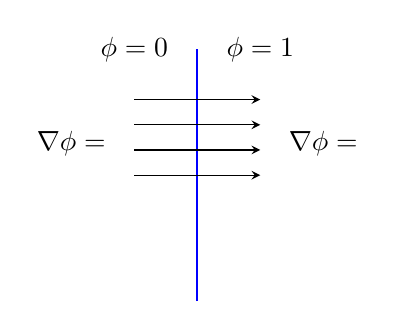
\begin{tikzpicture}[x={(0.8cm,0cm)}, y={(0cm,0.8cm)}, z={(-3.85mm, -3.85mm)}]
\def\rayon{3}
%styledesnœuds
\tikzstyle{textLine}=[rectangle, text=black]
\tikzstyle{textw}=[rectangle, text=black]
\tikzstyle{pointx}=[circle, fill, scale=0.2]
\tikzstyle{vector}=[-stealth,thin]


%planar interface
\coordinate (p0) at (-1,0);
\coordinate (p1) at (-90:2);
\coordinate (p2) at (90:2);
\coordinate (mid) at ($(p1)!0.5!(p2)$);
\draw[thick,blue] (p1) -- (p2);

\node[textLine, text centered] (chg) at ($(p2)-(1,0)$) { $\phi=0$};
\node[textLine, text centered] (chg) at ($(p2)+(1,0)$) { $\phi=1$};
\node[textLine, text centered] (chg) at ($(mid)-(2,-0.5)$) { $\nabla\phi=$};
\node[textLine, text centered] (chg) at ($(mid)+(2,0.5)$) { $\nabla\phi=$};
% %normal vector
\draw[vector] ($(p1)!0.5!(p2)-(1,0)$) -- ($(p1)!0.5!(p2)+(1,0)$);
\draw[vector] ($(p1)!0.6!(p2)-(1,0)$) -- ($(p1)!0.6!(p2)+(1,0)$);
\draw[vector] ($(p1)!0.7!(p2)-(1,0)$) -- ($(p1)!0.7!(p2)+(1,0)$);
\draw[vector] ($(p1)!0.8!(p2)-(1,0)$) -- ($(p1)!0.8!(p2)+(1,0)$);

\end{tikzpicture}



